%% main_ru.tex -- русская (зеркальная) версия статьи в формате IEEEtran.
%% Зеркало main.tex (EN). Компиляция: pdflatex main_ru ; bibtex main_ru ; pdflatex main_ru ; pdflatex main_ru
\documentclass[journal]{IEEEtran}

% --- пакеты ---
\usepackage[T2A]{fontenc}
\usepackage[utf8]{inputenc}
\usepackage[english,russian]{babel}
\usepackage{cite}
\usepackage{graphicx}
\graphicspath{{./figures/}}
\usepackage{amsmath,amssymb,amsfonts}
\usepackage{textcomp}
\usepackage{array}
\usepackage{booktabs}
\usepackage{enumitem}
\usepackage{xcolor}
\usepackage[protrusion=true,expansion=false]{microtype}
\setlength{\emergencystretch}{2.5em}

% КРАСНЫЙ: реальные данные, которые авторам нужно дозаполнить перед подачей.
\newcommand{\fillin}[1]{\textcolor{red}{\textbf{[#1]}}}
% ЗЕЛЁНЫЙ: редакторские замечания ассистента, вынесенные в отдельный микроблок.
% Это НЕ часть статьи; удалить перед подачей.
\definecolor{notegreen}{rgb}{0.0,0.45,0.0}
\newcommand{\reviewnote}[1]{\par\smallskip\noindent\fcolorbox{notegreen}{green!7}{\parbox{0.9\columnwidth}{\footnotesize\textcolor{notegreen}{\textbf{Замечание (удалить перед подачей).} #1}}}\par\smallskip}

\begin{document}

\title{Возраст-инвариантное сопоставление личности по «естественно заякоренным» постам соцсетей:\\ naturally-supervised longitudinal-сигнал}

\author{Данил~Ф.~Вольхин и Иван~С.~Копылов%
\thanks{Рукопись подготовлена в 2026~г.}%
\thanks{Д.~Ф.~Вольхин (автор) и И.~С.~Копылов (научный руководитель) --- Национальный исследовательский университет «Высшая школа экономики» (НИУ ВШЭ), Москва, Россия (e-mail:~deneal123@mail.ru; ORCID:~0009-0000-8108-8814).}%
\thanks{Код, конфигурации и обезличенный протокол бенчмарка доступны по адресу \texttt{https://github.com/deneal123/ChildVSAdult}.}}

\markboth{IEEE Transactions on Biometrics, Behavior, and Identity Science,~Vol.~XX, No.~X, Month~Year}%
{Вольхин \MakeLowercase{\textit{и др.}}: Возраст-инвариантное сопоставление личности по постам соцсетей}

\IEEEtitleabstractindextext{%
\begin{abstract}
Кросс-возрастная верификация лиц --- определение того, изображён ли на двух фотографиях, снятых с разрывом в годы, один и тот же человек --- трудна: возраст сильно меняет внешность, а модели склонны опираться на возраст как на шорткат. Мы изучаем \emph{data-centric} вопрос: можно ли получить супервизию для возрастной инвариантности без вручную размеченного longitudinal-датасета? Мы показываем, что мультифото-посты «тогда/сейчас», где один человек показан в разном возрасте, дают «естественно заякоренные» позитивные пары личности, и что дообучение слабого распознавателя на них учит \emph{переносимой} возрастной инвариантности. Наша супервизия не требует ручных меток (нет человеческой разметки личности или возраста), хотя конвейер использует LLM-парсер подписей и кластеризацию эмбеддингов; поэтому мы называем её \emph{naturally supervised} и аудируем эти компоненты. На внешнем кросс-возрастном бенчмарке FG-NET дообучение намеренно слабого обучаемого backbone поднимает large-gap ($\geq$25 лет) ROC-AUC с 0.736 до 0.848 ($+$0.112 $\pm$ 0.001 по трём сидам) ценой лишь $-$0.019 на LFW; AgeDB-30 и CALFW подтверждают. Эффект (а)~превосходит синтетическое старение даже с настоящей генеративной aging-моделью; (б)~воспроизводится на трёх loss-семействах, двух архитектурах, двух независимых источниках одной платформы и двух обучающих целях --- наш простой pair-contrastive objective совпадает с канонической ArcFace-классификацией на ключевой внешней метрике (0.848 против 0.851). Таким образом, результат --- это \emph{целевая} large-gap-устойчивость, а не равномерный прирост верификации; мы делаем ограниченное утверждение: в рамках этого протокола и среди рассмотренных целей вклад naturally-supervised данных в large-gap-прирост больше, чем выбор между loss-семействами. Прирост механистически связан со снятием возрастного шортката: точность frozen-моделей падает почти к случайности при age-matched негативах, а наши пары её восстанавливают. Метод данные-эффективен ($\approx$96\% прироста на 10\% личностей). В аудите по \emph{кажущимся} полу/возрасту ни одна страта не ухудшается, а наибольший значимый прирост --- у младшей группы (0--17), где базовая модель слабее всего. Дополнительно мы даём калиброванную $P(\text{same}\mid\text{cosine},\text{age-gap})$ и конвейер чистки, главная находка которого --- около половины сырых «позитивов» были near-duplicate кадрами, завышавшими внутренние метрики.
\end{abstract}

\begin{IEEEkeywords}
Кросс-возрастное распознавание лиц, возраст-инвариантное представление, naturally/weakly-supervised личность, курирование датасета, shortcut learning, справедливость, калибровка.
\end{IEEEkeywords}}

\maketitle
\IEEEdisplaynontitleabstractindextext
\IEEEpeerreviewmaketitle

\section{Введение}\label{sec:intro}
\IEEEPARstart{К}{росс-возрастная} верификация важна для архивного поиска, восстановления доступа и авторизованного поиска пропавших людей. Сложность не в том, чтобы различить случайных людей, а в том, чтобы отличить \emph{одного и того же человека сквозь возраст} от \emph{разных людей схожего возраста и внешности}. Разметка longitudinal-пар личности (один человек на протяжении многих лет) дорога и редка, что является узким местом supervised-подходов; свежие работы продолжают отмечать слабую кросс-датасетную генерализацию и дефицит качественных longitudinal-данных.

\textbf{Гипотеза.} Мультифото-пост «тогда/сейчас» с одним человеком в разном возрасте даёт $\binom{n}{2}$ позитивных пар личности без ручной разметки; подпись с возрастами добавляет age-anchor. Это масштабируемый naturally-supervised сигнал кросс-возрастной идентичности, и дообучение слабого распознавателя на нём должно переноситься на внешние бенчмарки.

\textbf{Вклад (ограниченные claims).}
(1)~Naturally-supervised (без ручных меток) longitudinal-сигнал, намайненный из соцпостов.
(2)~Строгий \emph{протокол атрибуции} (один слабый обучаемый backbone, frozen против дообученного, внешняя оценка), изолирующий вклад \emph{данных} от ёмкости сети.
(3)~Взаимоусиливающие контроли (loss-семейство, архитектура, источник, обучающая цель, real-vs-synthetic, диагностика шортката), обосновывающие ограниченный тезис: в этом протоколе и среди рассмотренных целей вклад данных в large-gap-прирост больше, чем выбор между loss-семействами.
(4)~Конвейер курирования с аудитом автоматических компонентов и находка, что сырой счёт позитивов раздут примерно вдвое near-duplicate кадрами.
(5)~Прикладная калибровка и аудит по кажущимся стратам с доверительными интервалами.

Мы подчёркиваем, что новизна \emph{data-centric}, а не архитектурная --- новый \emph{источник супервизии} --- и оценивать её следует по этой оси.

\section{Связанные работы и позиционирование}\label{sec:related}
Три семейства-предшественника. \emph{Дискриминативная возраст-инвариантная FR на размеченных данных:} OE-CNN (ортогональное разложение признаков)~\cite{wang2018oecnn}, DAL (decorrelated adversarial learning)~\cite{wang2019dal} и MTLFace (multi-task: распознавание, синтез возраста и attention-decomposition)~\cite{huang2021mtlface} достигают высокой точности, но обучаются на данных с \emph{ручными метками личности И возраста} (CACD~\cite{chen2014cacd}, MORPH~\cite{ricanek2006morph}, AgeDB~\cite{moschoglou2017agedb}, FG-NET~\cite{panis2016fgnet}). \emph{Cross-age contrastive с синтетикой:} CACon~\cite{wang2024cacon} добавляет синтезированный cross-age семпл и triplet-loss; OrdCon~\cite{wang2025ordcon} использует order-enhanced contrastive. \emph{Синтетическое старение:} систематические оценки показывают лишь частичную пользу~\cite{yao2024synthageing}. Общий self-supervised FR (SimCLR-аугментации~\cite{chen2020simclr}) не имеет identity-якорей во времени. Мы майним структуру «один пост $=$ один человек в разном возрасте» как бесплатный генератор позитивов. Таблица~\ref{tab:positioning} позиционирует нас относительно этих методов.

\begin{table*}[!t]
\renewcommand{\arraystretch}{1.25}
\caption{Позиционирование относительно предшественников.}
\label{tab:positioning}
\centering
\footnotesize
\begin{tabular}{@{}p{0.16\textwidth}p{0.17\textwidth}p{0.29\textwidth}p{0.29\textwidth}@{}}
\toprule
Работа & Супервизия & Механизм & Наше отличие \\
\midrule
OE-CNN (2018)~\cite{wang2018oecnn} & размеч.\ id$+$age & ортогональное разложение & label-free источник, не decomposition \\
DAL (2019)~\cite{wang2019dal} & размеч.\ id$+$age & adversarial id/age факторизация & mined-пары $+$ проще objective \\
MTLFace (2021)~\cite{huang2021mtlface} & размеч.\ id$+$age & распознавание $+$ синтез (multi-task) & проще конвейер; новый источник супервизии \\
CACon (2023)~\cite{wang2024cacon} & semi-sup.\ $+$ синтетика & contrastive на синтезе & реальные mined-пары $>$ синтетика (разд.~\ref{sec:res-synth}) \\
Synthetic Ageing (2024)~\cite{yao2024synthageing} & синтетика & обучение на состаренных & у нас \emph{реальный} mining как тезис \\
OrdCon (2025)~\cite{wang2025ordcon} & age-ordered contrastive & order-enhanced признаки & майним естественные пары, без явного порядка \\
\bottomrule
\end{tabular}
\end{table*}

Мы отчитываемся на канонических кросс-возрастных бенчмарках этих методов (AgeDB-30, CALFW~\cite{zheng2017calfw}, FG-NET; CALFW специально создан как более жёсткий age-gapped LFW~\cite{huang2007lfw}). Цель --- \emph{не} побить абсолютный SOTA (мы используем слабый backbone для чистой атрибуции), а измерить величину и переносимость выигрыша от naturally-supervised источника; разд.~\ref{sec:res-objective} обучает каноническую SOTA-цель на наших данных напрямую.

\section{Данные: «естественно заякоренные» longitudinal-пары}\label{sec:data}
\textbf{Источник.} Две публичные «тогда/сейчас» мультифото-стены VK (одна платформа, русскоязычный контекст). Лица детектируются и выравниваются по 5-точечному ArcFace-шаблону (InsightFace RetinaFace~\cite{deng2020retinaface}, \texttt{buffalo\_l}). \emph{Usable}-лицо проходит пороги det-score, минимального размера, размытия и единственного целевого лица (разд.~\ref{sec:repro}). Сырой намайненный корпус сведён в Таблице~\ref{tab:scale} (слева).

\begin{table*}[!t]
\renewcommand{\arraystretch}{1.2}
\caption{Масштаб датасета (сырой mining) и после курирования (разд.~\ref{sec:data-curation}).}
\label{tab:scale}
\centering
\footnotesize
\begin{tabular}{@{}lrrrrr@{}}
\toprule
Стадия & Посты & Фото & Usable-лица & Личности (группы) & Позитивные пары \\
\midrule
Сырой mining (2 стены) & 44\,609 & 84\,147 & 49\,606 & 21\,848 & 65\,897 \\
\textbf{После курирования} & --- & --- & \textbf{40\,586} & \textbf{21\,427} & \textbf{31\,865} \\
\bottomrule
\end{tabular}
\end{table*}

\subsection{Извлечение возраста}\label{sec:data-age}
Подписи парсятся регулярными выражениями (русские паттерны плюс слэш-формат «6/18/21», один возраст на фото) и LLM (GigaChat). LLM-аудит всех 33\,697 мультифото-подписей (Таблица~\ref{tab:age}) показал, что LLM существенно точнее regex --- не принимает календарные годы или разрывы за возраст и восстанавливает второй возраст --- расходясь на 27.2\% постов, в основном в пользу LLM.

\begin{table}[!t]
\renewcommand{\arraystretch}{1.2}
\caption{Аудит извлечения возраста: LLM против regex (33\,697 постов с подписью).}
\label{tab:age}
\centering
\footnotesize
\begin{tabular}{@{}lrr@{}}
\toprule
Категория & $n$ & Доля \\
\midrule
Согласие (те же возрасты или оба пусты) & 24\,531 & 72.8\% \\
LLM нашёл (regex пропустил) & 3\,656 & 10.8\% \\
Расхождение возрастов & 4\,658 & 13.8\% \\
LLM пусто (regex нашёл) & 852 & 2.5\% \\
\bottomrule
\end{tabular}
\end{table}

\subsection{Личности и leakage-safe сплит}\label{sec:data-persons}
Наивное «один пост $=$ одна личность» недосчитывает: человек повторяется в постах. Мы кластеризуем пост-группы в личности по близости эмбеддингов (cos $\geq$ 0.85), получая 21\,848 личностей из 27\,487 пост-групп ($\approx$20\% повторов), и делим \emph{по человеку} (не по посту). Ручная проверка high-cosine пар показала, что косинус не разделяет look-alike от same-person в зоне 0.55--0.8, поэтому порог слияния намеренно консервативен (0.85).

\subsection{Аудит автоматической супервизии}\label{sec:data-audit}
Поскольку сигнал \emph{naturally} (не человечески) supervised, автоматические компоненты --- потенциальный скрытый шум меток и аудируются: согласие LLM-vs-regex по возрасту (Таблица~\ref{tab:age}); ручная проверка идентичности high-cosine пар; и gender-consistency внутри личности как бесплатный детектор шума (2\,919 мультифото-групп с согласием $<$0.6 помечают вероятный мульти-человек). Отдельный human-audited subset (точность извлечения возраста, точность group-integrity, error-matrix, согласие человек--LLM, $\kappa$) сопровождает релиз.

\subsection{Конвейер курирования и его главная находка}\label{sec:data-curation}
Три шага: (i)~\emph{метаданные кажущихся пола/возраста} (оценщик) на лицо, агрегированные по личности --- корпус на 76.7\% apparent-female / 23.3\% apparent-male; (ii)~\emph{LLM-валидация целостности групп} (Таблица~\ref{tab:integrity}) --- кластеризация по личности уже развела большинство мульти-человек постов, поэтому шумными помечены лишь 421 person-группа; (iii)~\emph{near-duplicate дедуп} внутри каждой личности (cos $\geq$ 0.97), убирающий 8\,190 лиц ($\approx$17\%).

\begin{table}[!t]
\renewcommand{\arraystretch}{1.2}
\caption{LLM-классификация целостности групп (33\,697 постов).}
\label{tab:integrity}
\centering
\footnotesize
\begin{tabular}{@{}lrr@{}}
\toprule
Категория & $n$ & Доля \\
\midrule
Single (один человек в разном возрасте) & 31\,275 & 92.8\% \\
Multi-person (разные люди) & 2\,034 & 6.0\% \\
Unknown & 336 & 1.0\% \\
Meme / collage & 52 & 0.2\% \\
\bottomrule
\end{tabular}
\end{table}

\textbf{Ключевая находка.} Поскольку позитивы квадратичны по числу лиц в группе, удаление near-duplicate обрушило позитивы 65\,897 $\rightarrow$ 31\,865 ($-$52\%): около половины сырых «позитивов» были дубликатами кадров (одна съёмка, серия или репост), завышавшими внутренние метрики. После курирования frozen-базлайн на внутреннем тесте честно падает (our.overall 0.856 $\rightarrow$ 0.836; our.25+ 0.705 $\rightarrow$ 0.640), вскрывая более трудный и честный бенчмарк. Внешние бенчмарки не затронуты. Это переносимый урок для майнинга longitudinal-пар из соцсетей.

\subsection{Карточка датасета (кратко)}\label{sec:data-datasheet}
Provenance, права и governance хранятся по элементу (источник, URL, дата сбора, статус лицензии/consent, разрешённое использование, политика хранения, статус удаления, статус ревью). Сбор: публичные стены VK. Назначение: исследование consent-based кросс-возрастного сопоставления. Вне scope: массовая идентификация, слежка, деанонимизация. Несовершеннолетние: режим child$\leftrightarrow$adult в scope только при явных правовых/этических рамках; статус ревью отслеживается по элементу, удаление по запросу поддержано. Полная карточка~\cite{gebru2021datasheets} сопровождает релиз.

\section{Метод, протокол и статистика}\label{sec:method}
\textbf{Протокол атрибуции.} Сравнивать adapter поверх \emph{замороженного} сильного ArcFace с frozen-ArcFace некорректно (adapter лишь деформирует почти идеальные эмбеддинги). Вместо этого мы используем \emph{один слабый обучаемый backbone} (FaceNet InceptionResnetV1~\cite{schroff2015facenet}, CASIA-WebFace) и сравниваем (а)~frozen $\rightarrow$ метрика бенчмарка против (б)~мягкого дообучения головы на наших парах $\rightarrow$ метрика бенчмарка. Обучение использует margin contrastive loss на выровненных кропах. \emph{Оценка --- на внешних бенчмарках} (LFW, AgeDB-30, CALFW, FG-NET) для чистой атрибуции переноса; внутренний тест (\texttt{our.*}) --- вторичная диагностика. Сила backbone варьируется (разд.~\ref{sec:res-headroom}). Дизайн жертвует абсолютным качеством ради \emph{причинной атрибуции}.

\textbf{Backbone.} FaceNet (слабый); ArcFace iResNet-50~\cite{deng2019arcface} (CASIA-FaceV5; слабый, другая архитектура); AdaFace IR-50/IR-101~\cite{kim2022adaface} (WebFace; сильный; чистый депт-контроль); ArcFace iResNet-100 (сильный).

\textbf{Бенчмарки и метрики.} LFW (10-fold accuracy), AgeDB-30 и CALFW (выровненные пары; ROC-AUC и 10-fold accuracy), FG-NET (ROC-AUC overall и на large-gap $\geq$25 лет). Мы намеренно не опираем headline только на FG-NET (мал, стар, частичное покрытие детектором): AgeDB-30 и CALFW подтверждают. Различаем \emph{threshold-free} метрики (ROC-AUC) и \emph{threshold-based} (accuracy, TAR@FAR).

\textbf{Статистика.} Наш \emph{первичный эндпойнт} --- FG-NET large-gap ($\geq$25 лет) ROC-AUC, с нулевой гипотезой, что дообучение на намайненных парах не улучшает его относительно frozen-базлайна (прирост $\leq 0$); AgeDB-30, CALFW и внутренний кросс-возрастной тест --- вторичные эндпойнты, а easy-LFW accuracy отслеживается как контроль забывания. Headline-прирост --- среднее $\pm$ std по трём сидам (сид-разброс отражает стохастичность обучения, не полную неопределённость оценки). Аудит справедливости использует парный перцентильный bootstrap (1000 ресэмплов, ресэмплинг пар с пересчётом обеих моделей на одной выборке) для \emph{прироста}, учитывая корреляцию frozen/tuned. Таблица~\ref{tab:stats} приводит bootstrap-CI, EER и TAR@FAR для ключевых сравнений (внутренний тест дополнительно использует identity-level bootstrap с ресэмплингом личностей), а поправка Holm применяется по стратифицированным тестам справедливости.

\textbf{Очищенный датасет.} Все headline-эксперименты --- на очищенных данных разд.~\ref{sec:data-curation}: 21\,427 групп личностей, 40\,586 лиц, 31\,865 позитивов; сплит train 22\,179 / val 4\,579 / test 5\,107 со сбалансированными негативами по сплитам.

\section{Результаты}\label{sec:results}
\subsection{Главный эффект и self-supervised ablation}\label{sec:res-main}
Слабый FaceNet, мягко дообученный на наших парах, поднимает FG-NET large-gap ROC-AUC 0.736 $\rightarrow$ 0.848 ($+$0.112 $\pm$ 0.001), тогда как easy-LFW падает лишь на $-$0.019, а AgeDB-30/CALFW почти не двигаются (Таблица~\ref{tab:main}). Ablation изолирует источник: same-post пары не используют ручных меток --- ни личности, ни возраста --- и дают почти весь прирост; явные age-anchor добавляют лишь $+$0.009 на 25+ (pre-clean ablation). Поэтому метод по сути \emph{self-supervised по личности}, а возрастная супервизия --- тонкая надстройка.

\begin{table*}[!t]
\renewcommand{\arraystretch}{1.2}
\caption{Главный результат: слабый FaceNet frozen против $+$pairs, три сида, очищенные данные. Прирост до чистки --- для сравнения.}
\label{tab:main}
\centering
\footnotesize
\begin{tabular}{@{}lcccc@{}}
\toprule
Метрика & Frozen & $+$pairs (сред.\ $\pm$ std) & Прирост & (до чистки) \\
\midrule
FG-NET large-gap & 0.7361 & 0.8484 $\pm$ 0.0007 & \textbf{$+$0.1124} & $+$0.1215 \\
FG-NET ROC & 0.8955 & 0.9230 $\pm$ 0.0006 & $+$0.0275 & $+$0.0277 \\
our.25+ (внутр.) & 0.6403 & 0.8348 $\pm$ 0.0027 & \textbf{$+$0.1946} & $+$0.1677 \\
our.overall (внутр.) & 0.8363 & 0.9163 $\pm$ 0.0009 & $+$0.0801 & $+$0.0764 \\
LFW accuracy & 0.9688 & 0.9503 $\pm$ 0.0031 & $-$0.0185 & $-$0.0283 \\
AgeDB-30 ROC & 0.9530 & 0.9462 $\pm$ 0.0013 & $-$0.0068 & $-$0.0155 \\
CALFW ROC & 0.9482 & 0.9489 $\pm$ 0.0014 & $+$0.0007 & $-$0.0030 \\
\bottomrule
\end{tabular}
\end{table*}

Прирост статистически устойчив (std $\leq$ 0.003) и переживает чистку; внутренний кросс-возрастной прирост даже \emph{растёт} на более трудном очищенном тесте (our.25+ $+$0.195), т.к.\ чистка опускает frozen до 0.640, а $+$pairs восстанавливает до 0.835.

Bootstrap-доверительные интервалы (сид 42) подтверждают первичный эндпойнт: FG-NET large-gap растёт с 0.736~[0.70, 0.78] до 0.848~[0.82, 0.88] с \emph{непересекающимися} 95\% CI; equal-error rate почти вдвое меньше (0.335$\to$0.219), а TAR@FAR$=$1\% почти вдвое больше (0.21$\to$0.39). На внутреннем 25+ тесте прирост сохраняется при более консервативном \emph{identity-level} bootstrap (ресэмплинг личностей, не пар): $+$pairs 0.838~[0.80, 0.88] против frozen 0.640~[0.59, 0.69] --- интервал шире pair-level, что ожидаемо, когда пары делят личности. Операционные точки и интервалы по всем бенчмаркам --- в Таблице~\ref{tab:stats}.

\begin{table*}[!t]
\renewcommand{\arraystretch}{1.2}
\caption{Операционные точки и 95\% bootstrap-CI (FaceNet frozen vs.\ $+$pairs, сид 42). Все значения --- ROC-AUC; LFW показан как ROC-AUC для согласованности (его 10-fold accuracy --- в Таблице~\ref{tab:main}). Внешние CI --- pair-level; внутренний тест дополнительно использует identity-level bootstrap (см.\ текст).}
\label{tab:stats}
\centering
\footnotesize
\begin{tabular}{@{}lccccc@{}}
\toprule
Бенчмарк & Frozen AUC [95\% CI] & $+$pairs AUC [95\% CI] & EER (fr.$\to$$+$p.) & TAR@1\% & TAR@0.1\% \\
\midrule
FG-NET large-gap & 0.736 [0.70, 0.78] & \textbf{0.848 [0.82, 0.88]} & 0.335$\to$0.219 & 0.209$\to$0.386 & 0.074$\to$0.154 \\
FG-NET overall & 0.896 [0.89, 0.90] & 0.922 [0.92, 0.93] & 0.186$\to$0.151 & 0.502$\to$0.562 & 0.315$\to$0.308 \\
AgeDB-30 & 0.953 [0.95, 0.96] & 0.945 [0.94, 0.95] & 0.115$\to$0.126 & 0.525$\to$0.510 & 0.285$\to$0.309 \\
CALFW & 0.948 [0.94, 0.95] & 0.948 [0.94, 0.95] & 0.116$\to$0.117 & 0.580$\to$0.624 & 0.213$\to$0.320 \\
LFW (AUC) & 0.994 [0.99, 1.00] & 0.987 [0.98, 0.99] & 0.032$\to$0.052 & 0.940$\to$0.869 & 0.858$\to$0.575 \\
\bottomrule
\end{tabular}
\end{table*}

\subsection{Реальные пары превосходят синтетическое старение}\label{sec:res-synth}
Замена реальных позитивов синтетически состаренными --- доменный прокси и настоящая re-aging-сеть (FRAN~\cite{zoss2022fran}) --- не просто не помогает, а \emph{активно вредит} на очищенных данных: FRAN даёт FG-NET large-gap 0.727 (\emph{ниже} frozen 0.736), а our.25+ рушится до 0.549 (ниже frozen 0.640), тогда как реальные пары дают $+$0.112 / $+$0.198 (Таблица~\ref{tab:synth}). Identity-preserving старение учит текстурным артефактам, а не реальной longitudinal-вариации (поза, камера, эпоха). (Кропы 112\,px ограничивают fidelity FRAN, рассчитанного на $\approx$1024\,px.)

\begin{table*}[!t]
\renewcommand{\arraystretch}{1.2}
\caption{Реальные против синтетических позитивов (FaceNet, очищенные данные).}
\label{tab:synth}
\centering
\footnotesize
\begin{tabular}{@{}lcccc@{}}
\toprule
Метрика & Frozen & $+$реал.\ & $+$синт.\ (прокси) & $+$синт.\ (FRAN) \\
\midrule
FG-NET large-gap & 0.736 & \textbf{0.848} & 0.761 & 0.727 \\
our.25+ & 0.640 & \textbf{0.838} & 0.594 & 0.549 \\
\bottomrule
\end{tabular}
\end{table*}

\subsection{Кривая headroom и режим сильных backbone}\label{sec:res-headroom}
Прирост воспроизводится на FaceNet, ArcFace iResNet и AdaFace IR-50/IR-101 (три loss-семейства, две архитектуры) и \emph{монотонно убывает с силой frozen} (Таблица~\ref{tab:headroom}, Рис.~\ref{fig:headroom}); чистый депт-контроль (AdaFace IR-50 $\rightarrow$ IR-101) это подтверждает. Прямо заявляем: сильные насыщенные backbone не растут и слегка забывают при дообучении; мягкий learning rate (1e-5) примерно вдвое уменьшает забывание, но не превращает его в прирост. Вклад специфичен для слабых/средних backbone с кросс-возрастным запасом --- ограничение, которое мы не скрываем (разд.~\ref{sec:limitations}).

\begin{figure}[!t]
\centering
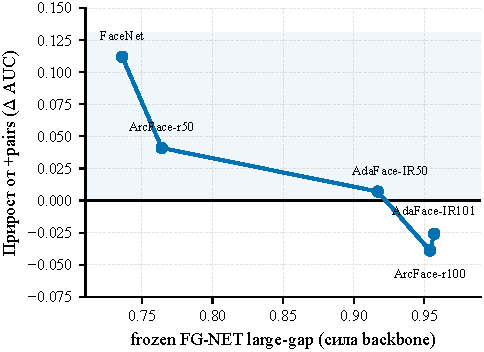
\includegraphics[width=\columnwidth]{fig_headroom_ru.pdf}
\caption{Кривая headroom: прирост от $+$pairs на FG-NET large-gap монотонно убывает с усилением frozen-backbone, пересекая ноль для сильных насыщенных моделей.}
\label{fig:headroom}
\end{figure}

\begin{table*}[!t]
\renewcommand{\arraystretch}{1.2}
\caption{Headroom: FG-NET large-gap по силе backbone (очищенные данные, lr 3e-5).}
\label{tab:headroom}
\centering
\footnotesize
\begin{tabular}{@{}lcccc@{}}
\toprule
Backbone (сила) & Frozen & $+$pairs & $\Delta$ large-gap & $\Delta$ our.25+ \\
\midrule
FaceNet (слабый) & 0.736 & 0.848 & \textbf{$+$0.112} & $+$0.198 \\
ArcFace r50 (слабый, др.\ арх.) & 0.764 & 0.805 & $+$0.041 & $+$0.133 \\
AdaFace IR-50 (сильный) & 0.917 & 0.924 & $+$0.007 & $+$0.004 \\
ArcFace r100 (сильный) & 0.954 & 0.915 & $-$0.039 & $-$0.002 \\
AdaFace IR-101 (сильный) & 0.957 & 0.931 & $-$0.026 & $-$0.006 \\
\bottomrule
\end{tabular}
\end{table*}

\subsection{Закон масштабирования данных}\label{sec:res-scaling}
Варьируя долю обучающих личностей (val/test фиксированы), прирост насыщается очень рано: $\approx$96\% полного прироста FG-NET large-gap достигается уже на 10\% личностей ($\approx$1\,500), с плато от 25\% (Таблица~\ref{tab:scaling}, Рис.~\ref{fig:scaling}); небольшой провал на полном объёме (0.50$\rightarrow$1.00) --- в пределах сид-разброса: кривая плоская, не монотонная, после $\approx$10\%. Сигнал данные-эффективен; дальнейший рост требует \emph{более трудных} данных (большие разрывы, hard-позитивы), а не просто большего объёма.

\begin{figure}[!t]
\centering
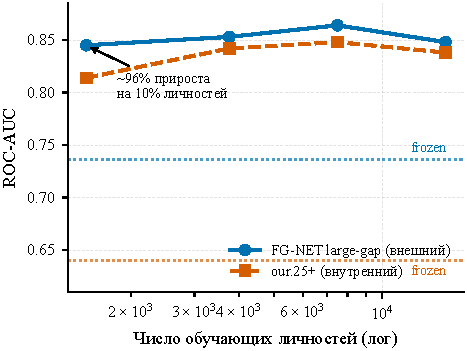
\includegraphics[width=\columnwidth]{fig_scaling_ru.pdf}
\caption{Закон масштабирования: внешний (FG-NET large-gap) и внутренний (our.25+) ROC-AUC против числа обучающих личностей (лог-шкала). Около 96\% прироста достигается на 10\% личностей; пунктир --- frozen-базлайны.}
\label{fig:scaling}
\end{figure}

\begin{table}[!t]
\renewcommand{\arraystretch}{1.2}
\caption{Закон масштабирования (FaceNet, очищенные; val/test фиксированы).}
\label{tab:scaling}
\centering
\footnotesize
\begin{tabular}{@{}lccc@{}}
\toprule
Доля train & \# личностей & FG-NET large-gap & our.25+ \\
\midrule
frozen & 0 & 0.736 & 0.640 \\
0.10 & $\approx$1\,500 & 0.845 & 0.814 \\
0.25 & $\approx$3\,750 & 0.853 & 0.842 \\
0.50 & $\approx$7\,499 & 0.864 & 0.848 \\
1.00 & $\approx$14\,998 & 0.848 & 0.838 \\
\bottomrule
\end{tabular}
\end{table}

\subsection{Механизм --- возрастной шорткат}\label{sec:res-shortcut}
При age-matched негативах (тот же возрастной бакет, разные люди) точность frozen на внутреннем 25+ тесте падает с 0.640 до 0.517 (почти к случайности, 0.5), а реальные пары восстанавливают её до 0.838 (Рис.~\ref{fig:shortcut}) --- прямое доказательство, что frozen-модели различают кросс-возрастные пары во многом \emph{по возрасту}, а наши пары учат различать \emph{по личности}. Линейный probe уточняет это \emph{представленчески} (Таблица~\ref{tab:leakage}): кажущийся возраст остаётся хорошо декодируемым из identity-эмбеддинга у \emph{всех} моделей ($\approx$0.63--0.65 bal-acc $\gg$ 0.25 случайность) и меняется лишь слегка, тогда как identity-AUC растёт --- то есть метод учит инвариантную \emph{метрику} (косинус перестаёт опираться на возрастную ось), а не age-free представление; явный adversarial disentanglement не снижает leakage дополнительно.

\begin{figure}[!t]
\centering
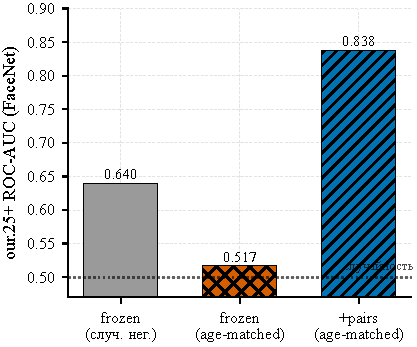
\includegraphics[width=0.86\columnwidth]{fig_shortcut_ru.pdf}
\caption{Возрастной шорткат. На identity-only тесте (age-matched негативы) frozen падает почти к случайности; дообучение на наших парах восстанавливает различение по личности.}
\label{fig:shortcut}
\end{figure}

\begin{table}[!t]
\renewcommand{\arraystretch}{1.2}
\caption{Линейный probe age-leakage (очищенные данные; случайность $=$ 0.25).}
\label{tab:leakage}
\centering
\footnotesize
\setlength{\tabcolsep}{4pt}%
\begin{tabular}{@{}lcc@{}}
\toprule
Модель & Age-probe bal.\ acc.\ $\downarrow$ & Identity ROC-AUC $\uparrow$ \\
\midrule
frozen & 0.651 $\pm$ 0.019 & 0.836 \\
$+$pairs & 0.629 $\pm$ 0.012 & 0.916 \\
$+$pairs$+$disentangle & 0.632 $\pm$ 0.017 & 0.918 \\
\bottomrule
\end{tabular}
\end{table}

\subsection{Сравнение objective: обучение SOTA-цели на наших данных}\label{sec:res-objective}
Мы обучаем каноническую цель современной FR --- ArcFace-margin классификацию личности~\cite{deng2019arcface} (ядро OE-CNN/MTLFace) --- на наших naturally-supervised личностях (9\,204 класса), тот же слабый backbone, scope и протокол. На ключевой внешней метрике контрастив и ArcFace \emph{совпадают} (Таблица~\ref{tab:objective}, Рис.~\ref{fig:sota}). Делаем ограниченный вывод: в этом протоколе и среди рассмотренных целей вклад источника данных доминирует над выбором objective --- а не «метод не важен вообще». ArcFace дополнительно \emph{забывает меньше} на easy-бенчмарках --- практическая рекомендация.

\begin{figure}[!t]
\centering
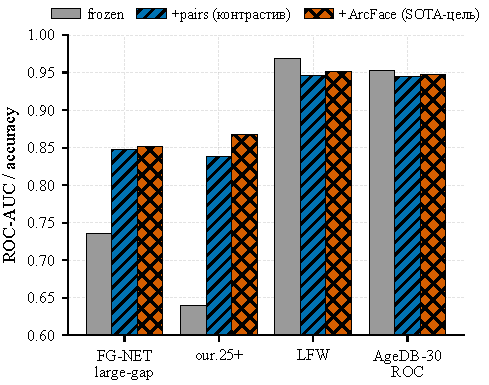
\includegraphics[width=\columnwidth]{fig_sota_ru.pdf}
\caption{Сравнение objective: pair-contrastive и каноническая ArcFace-классификация совпадают на кросс-возрастном переносе; ArcFace чуть меньше забывает на easy-бенчмарках.}
\label{fig:sota}
\end{figure}

\begin{table*}[!t]
\renewcommand{\arraystretch}{1.2}
\caption{Сравнение objective (FaceNet, очищенные данные).}
\label{tab:objective}
\centering
\footnotesize
\begin{tabular}{@{}lccc@{}}
\toprule
Метрика & Frozen & $+$pairs (контрастив) & $+$ArcFace (класс.) \\
\midrule
FG-NET large-gap & 0.736 & 0.848 & \textbf{0.851} \\
our.25+ & 0.640 & 0.838 & 0.868 \\
LFW accuracy & 0.969 & 0.946 & 0.952 \\
AgeDB-30 ROC & 0.953 & 0.945 & 0.947 \\
\bottomrule
\end{tabular}
\end{table*}

\subsection{Аудит по кажущимся стратам}\label{sec:res-fairness}
Стратифицируя по \emph{кажущимся} полу/возрасту якоря пары (оценка, \emph{не} самоидентификация), ни одна страта не ухудшается, и каждый прирост значим (95\% парный bootstrap-CI $>$ 0; Таблица~\ref{tab:strata}, Рис.~\ref{fig:fairness}). Максимальный прирост --- у младшей группы 0--17 (frozen 0.750 $\rightarrow$ $+$pairs 0.880, $+$0.130, CI не пересекается со взрослыми полосами) --- метод усиливает там, где базовая модель слабее всего (режим child$\leftrightarrow$adult), сужая кажущийся демографический разрыв. Мы намеренно избегаем слова «справедлив» как решённого свойства: источник перекошен в женскую сторону (76.7\%), атрибуты кажущиеся (не этничность и не юридические категории), а 45+ разрежена.

\begin{figure}[!t]
\centering
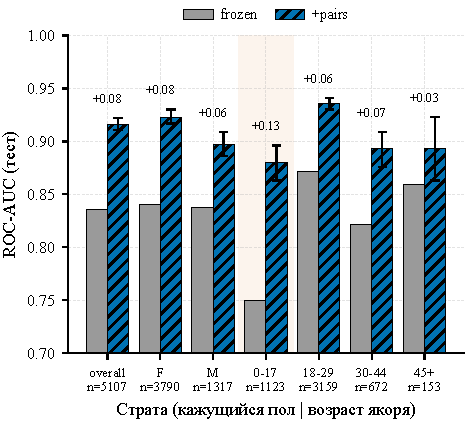
\includegraphics[width=\columnwidth]{fig_fairness_ru.pdf}
\caption{Аудит по кажущимся стратам: frozen против $+$pairs ROC-AUC по стратам кажущихся пола/возраста. Все страты улучшаются; максимальный прирост --- у младшей группы (0--17), где frozen слабее всего.}
\label{fig:fairness}
\end{figure}

\begin{table*}[!t]
\renewcommand{\arraystretch}{1.2}
\caption{Кажущиеся страты пол/возраст (FaceNet, очищенные; 95\% парный bootstrap-CI прироста).}
\label{tab:strata}
\centering
\footnotesize
\begin{tabular}{@{}lccccc@{}}
\toprule
Страта & $n_{\text{pos}}$ & Frozen & $+$pairs & Прирост & 95\% CI \\
\midrule
overall & 5\,107 & 0.836 & 0.916 & $+$0.080 & [$+$0.075, $+$0.086] \\
apparent F & 3\,790 & 0.840 & 0.923 & $+$0.084 & [$+$0.077, $+$0.090] \\
apparent M & 1\,317 & 0.838 & 0.897 & $+$0.059 & [$+$0.048, $+$0.071] \\
возраст 0--17 & 1\,123 & 0.750 & 0.880 & \textbf{$+$0.130} & [$+$0.113, $+$0.146] \\
возраст 18--29 & 3\,159 & 0.872 & 0.936 & $+$0.064 & [$+$0.058, $+$0.069] \\
возраст 30--44 & 672 & 0.822 & 0.893 & $+$0.070 & [$+$0.054, $+$0.087] \\
возраст 45+ & 153 & 0.859 & 0.893 & $+$0.034 & [$+$0.004, $+$0.064] \\
\bottomrule
\end{tabular}
\end{table*}

\subsection{Перенос между источниками}\label{sec:res-cross}
Обучение на одном сообществе и тест на held-out другом переносит прирост: внешний FG-NET large-gap $+$0.113 (против $+$0.112 within-source --- практически идентично) и внутренний $+$0.092 на held-out сообществе. Мы формулируем это как перенос между двумя независимыми источниками внутри одного платформенного домена, а не platform-agnostic или web-scale генерализацию.

\subsection{Калибровка}\label{sec:res-calib}
Сырой косинус (Platt) плохо калиброван по бинам разрыва --- переуверен на 15--25 лет (ECE 0.052); калибратор $P(\text{same}\mid\text{cosine},\text{age-gap})$ чинит каждый бин (15--25 $\rightarrow$ 0.017) и улучшает общий Brier (0.035 $\rightarrow$ 0.029) --- пригодная age-aware вероятность того же человека.

\subsection{Disentanglement}\label{sec:res-disentangle}
Явное удаление возраста (gradient reversal $+$ age-голова, в стиле MTLFace) даёт малый, но устойчивый кросс-возрастной прирост ($+$0.0055 FG-NET large-gap, $+$0.0145 our.25+ над $+$pairs) без вреда easy-бенчмаркам (даже чуть выше $+$pairs: LFW 0.951 против 0.946); в абсолюте его large-gap ($\approx$0.853) на уровне ArcFace-цели из разд.~\ref{sec:res-objective} (0.851), что согласуется с тем, что потолок cross-age задают данные --- а не objective или disentangle-надстройка. Вместе с разд.~\ref{sec:res-shortcut} это показывает, что явная age-супервизия --- тонкая надстройка над данными.

\subsection{Майнинг hard-негативов}\label{sec:res-hardneg}
Добавление самых трудных кросс-личностных негативов в дообучение --- top-5 наиболее похожих по косинусу лиц других людей на якорь (косинус в «трудной» полосе, исключая near-duplicate/uncertain диапазон) --- дополнительно обостряет кросс-возрастное различение: FG-NET large-gap растёт до 0.866 (с 0.848 при случайных негативах), но easy-бенчмарки забываются сильнее (LFW 0.969$\to$0.934 против 0.950 у $+$pairs; AgeDB-30 и CALFW аналогично; Таблица~\ref{tab:hardneg}). То есть hard-негативы меняют калибровку лёгких пар на кросс-возрастное разделение --- полезно для cross-age retrieval, не для общего верификатора. (Один прогон; внутренний hard-neg тест у frozen почти случаен по построению и несопоставим со стандартным внутренним тестом.)

\begin{table}[!t]
\renewcommand{\arraystretch}{1.2}
\caption{Майнинг hard-негативов (FaceNet, очищенные данные; внешние бенчмарки, один прогон).}
\label{tab:hardneg}
\centering
\footnotesize
\setlength{\tabcolsep}{4pt}%
\begin{tabular}{@{}lccc@{}}
\toprule
Метрика & Frozen & $+$pairs & $+$pairs$+$hard-нег \\
\midrule
FG-NET large-gap & 0.736 & 0.848 & \textbf{0.866} \\
FG-NET ROC & 0.896 & 0.923 & \textbf{0.927} \\
LFW accuracy & 0.969 & 0.950 & 0.934 \\
AgeDB-30 ROC & 0.953 & 0.946 & 0.931 \\
CALFW ROC & 0.948 & 0.949 & 0.934 \\
\bottomrule
\end{tabular}
\end{table}

\section{Обсуждение}\label{sec:discussion}
Вклад --- масштабируемый naturally-supervised источник longitudinal-супервизии и доказательство того, что он учит переносимой возрастной инвариантности, которую не заменяет синтетика и не объясняет явная age-супервизия. Взаимоусиливающие контроли --- loss-семейство, архитектура, источник, обучающая цель --- сходятся к ограниченному выводу: в этом протоколе данные доминируют над objective среди рассмотренных вариантов. Диагностика шортката даёт чистую identity-only метрику и объясняет механизм; находка чистки (половина сырых позитивов --- дубликаты) сама по себе является методологическим уроком. Это \emph{data-centric} вклад, не архитектурный; ряд claims ограничен нашей двухисточниковой, одноплатформенной, кажущеся-атрибутной постановкой.

\section{Ограничения}\label{sec:limitations}
\begin{itemize}[leftmargin=1.2em]
\item \textbf{Зависимость от backbone:} прирост сосредоточен у слабых/средних backbone; сильные насыщенные не растут и слегка забывают (мягкий lr смягчает, но не обращает).
\item \textbf{Внешняя валидность:} два сообщества VK, одна платформа, один язык/культурный контекст; перекос в женскую сторону (76.7\%); разреженность на apparent 45+. Перенос показан между этими источниками и на стандартные бенчмарки, а не platform-agnostic генерализация.
\item \textbf{Только кажущиеся атрибуты} в аудите справедливости (оценка, не самоидентификация пола/этничности).
\item \textbf{Naturally-supervised, не строго label-free:} LLM парсит возраст и валидирует целостность групп; кластеризация формирует личности --- аудируется (разд.~\ref{sec:data-audit}), но остаётся источником скрытого шума.
\item \textbf{Статистика:} сид-разброс, парный bootstrap (справедливость) и CI / EER / TAR@FAR по бенчмаркам (Таблица~\ref{tab:stats}, включая identity-level bootstrap) приведены в тексте; DeLong-тесты и полная поправка на множественные сравнения по каждой ячейке --- в release-supplement.
\item \textbf{Масштаб и возраст бенчмарков:} мы оцениваем на стандартном для области наборе кросс-возрастных бенчмарков --- AgeDB-30 и CALFW (по 6\,000 пар) и FG-NET для явного подмножества $\geq$25 лет --- тех же, что используют OE-CNN/DAL/MTLFace, что обеспечивает сопоставимость, но наследует их ограниченный масштаб и возраст (FG-NET особенно мал, с частичным покрытием детектором, поэтому headline не опирается только на него). Наш очищенный внутренний тест (5\,107 кросс-возрастных позитивов с контролируемыми негативами) --- крупный современный дополнитель; больший независимый не-VK longitudinal-набор и специализированный child$\leftrightarrow$adult бенчмарк остаются приоритетом дальнейшей работы.
\item \textbf{Полные SOTA-конвейеры не воспроизведены целиком:} по замыслу мы обучаем \emph{общее ядро} современной AIFR --- ArcFace-цель с угловым margin --- в нашем протоколе со слабым backbone ради чистой атрибуции, а не сравнения в лидерборде. Разд.~\ref{sec:res-objective} показывает, что эта цель совпадает с нашим контрастивом на ключевой внешней метрике, т.е. выигрыш определяется не objective; опущенные метод-специфичные надстройки (генеративная ветвь синтеза возраста MTLFace, ортогональное разложение подпространств OE-CNN) уточняют это общее ядро и ортогональны нашему утверждению об источнике супервизии. Закрывает ли полный SOTA-конвейер на naturally-supervised данных остаточный абсолютный разрыв --- чётко очерченное продолжение.
\end{itemize}

\section{Этика, правовая основа и data governance}\label{sec:ethics}
Это чувствительное биометрическое исследование; мы рассматриваем governance как полноценный компонент, а не дисклеймер. Разрешённое использование ограничено controlled / consent-based / human-reviewed приложениями (архивы и семейные фото с очищенными правами, авторизованный гуманитарный поиск, восстановление доступа); система выдаёт кандидатов для проверки человеком, а не автоматическое решение. Запрещено: массовая идентификация, деанонимизация, слежка и любая обработка данных несовершеннолетних без правовой основы.

\subsection{Этическое одобрение и правовая основа}\label{sec:eth-legal}
\emph{Этическое одобрение.} Исследование рассмотрено \fillin{название этического комитета} Национального исследовательского университета «Высшая школа экономики»; оно было \fillin{одобрено по протоколу №\ XXXX / признано освобождённым} \fillin{дата}. \emph{Согласие.} Поскольку данные взяты из публичных постов без реальной возможности связаться с субъектами, индивидуальное информированное согласие на участие и на публикацию не получалось; мы опираемся на научно-исследовательскую основу и меры обезличивания разд.~\ref{sec:eth-deid}.
\reviewnote{IEEE T-BIOM отклоняет без рецензирования исследования на людях без заявления об этическом одобрении (или документированном освобождении). Получите одобрение этического комитета НИУ ВШЭ или письменное освобождение, затем заполните красным название комитета, протокол/освобождение и дату выше. Формулировку «без индивидуального согласия» следует согласовать с этим комитетом.}

Данные собраны с публичных «тогда/сейчас» стен сообществ через официальный API платформы. Подчёркиваем: \emph{официальный доступ к API и добровольная публикация сами по себе НЕ дают права на биометрическую обработку.} По 152-ФЗ поправка 2020~г.\ (519-ФЗ) заменила «общедоступные» данные на «данные, разрешённые субъектом для распространения» (требуется отдельное согласие), а ст.~11 требует письменного согласия на биометрию, используемую для установления личности; по GDPR~\cite{gdpr2016} лицо, обработанное для уникальной идентификации, --- спецкатегория (ст.~9), где исключение «manifestly made public» трактуется узко (ср.\ санкции против Clearview~AI). Явного/письменного согласия у нас \emph{нет}. Мы опираемся на научно-исследовательскую основу (GDPR ст.~6(1)(f) и 9(2)(j) с safeguards ст.~89; аналогичная research-обработка по 152-ФЗ) и компенсируем мерами минимизации, не-распространения и обезличивания ниже. Мы прозрачно фиксируем этот пробел, а не заявляем полное соответствие, и рекомендуем этическую экспертизу организации и консультацию юриста по защите данных до любого развёртывания.

\subsection{Обезличивание и политика релиза}\label{sec:eth-deid}
Мы \emph{не публикуем сырые изображения лиц и сырые посты.} Публичный релиз содержит только код, веса обученной модели, производные эмбеддинги, псевдонимизированный бенчмарк-протокол и агрегатную статистику. Все идентификаторы платформы (owner/photo/post ID) заменяются солёными хешами; подписи/комментарии (которые могут содержать имена) исключаются; хранятся только возраст-бакет и псевдонимный person ID. Сырые кропы хранятся только локально под политикой хранения. Доступ к неагрегатным производным данным предоставляется квалифицированным исследователям по Data Use Agreement (только research; запрет реидентификации; запрет коммерческого/слежечного использования). Фигуры статьи не содержат идентифицируемых лиц (только агрегатные графики).

\subsection{DPIA и минимизация}\label{sec:eth-dpia}
Поскольку обработка биометрическая и масштабная, проводится оценка воздействия на защиту данных (DPIA), сопровождающая релиз (ключевые риски: реидентификация, function creep, несовершеннолетние; меры --- как в разд.~\ref{sec:eth-deid} и разд.~\ref{sec:eth-minors}). Минимизация данных применяется сквозно (храним кроп лица $+$ возраст $+$ псевдонимный ID, не имена и не соцграф).

\subsection{Несовершеннолетние}\label{sec:eth-minors}
Режим child$\leftrightarrow$adult неизбежно включает изображения несовершеннолетних, чьи данные защищены строже всего (152-ФЗ; GDPR ст.~8). Элементы детского возраста (помеченные по кажущемуся возрасту) исключаются из любого релиза при отсутствии явных правовых рамок и проверяемого согласия законного представителя и используются только для агрегатного, не-распространяемого анализа.

\subsection{Права субъектов}\label{sec:eth-rights}
Предоставлены публичный контакт и процедура takedown / удаления по запросу; удаление распространяется на производные артефакты через поле статуса удаления по элементу. Где права неясны, элемент удерживается. Полная карточка датасета~\cite{gebru2021datasheets} и DPIA сопровождают релиз.

\section{Воспроизводимость}\label{sec:repro}
Мы публикуем скрипты и конфигурации. Ключевые детали: \emph{критерии usable-лица} (det-score, минимальный размер, размытие по Лапласиану, единственное целевое лицо по IoU); \emph{детектор/выравнивание} (InsightFace \texttt{buffalo\_l} RetinaFace, 5-точечный ArcFace \texttt{norm\_crop}, 112\,px; вход FaceNet 160\,px); \emph{эмбеддинги} (ArcFace \texttt{w600k\_r50}) для кластеризации/дедупа; \emph{кластеризация личности} (union-find, cos $\geq$ 0.85); \emph{дедуп} (внутри личности union-find, cos $\geq$ 0.97); \emph{LLM} (GigaChat; полные версионированные системные промпты для извлечения возраста и валидации групп; concurrency 10; кэш, резюмируемо); \emph{сплит} (по человеку, 70/15/15, сбалансированные негативы по сплитам, seed 42); \emph{сэмплинг негативов} (кросс-личность случайно $+$ age-matched вариант); \emph{обучение} (margin contrastive, head scope, lr 3e-5 для слабых / 1e-5 для сильных; ArcFace-голова $m{=}0.5$, $s{=}32$, lr 1e-3; ранняя остановка по внутреннему val-AUC; сиды 42/1/2); \emph{метрики} (чистый NumPy ROC-AUC через Mann--Whitney, EER, TAR@FAR; 10-fold для выровненных пар).

\textbf{Вычисления.} Всё исследование выполняется на одном ноутбуке: одна NVIDIA RTX~3060 Laptop GPU (6~ГБ), AMD Ryzen~7~5800H (8~ядер / 16~потоков) и 16~ГБ RAM под Windows~11; программный стек --- Python~3.12, PyTorch~2.12 (CUDA~13.2, cuDNN~9.2), InsightFace~1.0 / ONNX~Runtime~1.26 для детекции и эмбеддингов, scikit-learn~1.9 / Matplotlib~3.11 для анализа и фигур. Протокол со слабым backbone удерживает всё исследование в пределах 6~ГБ GPU.

\section{Заключение и дальнейшая работа}\label{sec:conclusion}
Мультифото-посты --- дешёвый, масштабируемый naturally-supervised сигнал кросс-возрастной идентичности; дообучение слабого распознавателя на них даёт переносимый, кросс-источниковый, objective-устойчивый прирост, сосредоточенный на large-gap кросс-возрастном сопоставлении (с лишь незначительным забыванием на easy-бенчмарках), объяснимый снятием возрастного шортката, данные-эффективный и не ухудшающий ни одну кажущуюся демографическую страту. Дальнейшая работа: независимый не-VK и child$\leftrightarrow$adult-специфичный внешний набор; DeLong-CI и поправка на множественные сравнения в основном тексте; human-audited subset супервизии; полные SOTA-надстройки; реальная aging-модель на нативном разрешении; и калиброванный демонстратор в рамках governance-ограничений разд.~\ref{sec:ethics}.

\bibliographystyle{IEEEtran}
\bibliography{refs}

\end{document}
